\documentclass[letterpaper,11pt,twocolumn]{article}
\usepackage{fullpage}
\usepackage{color}
\usepackage{graphicx}
\usepackage{epsfig}
\usepackage{amsthm}
\usepackage{latexsym}
\usepackage{amssymb}
\usepackage{amsmath}

\newcommand{\newfontobj}[2]{
  \newcommand{#1}[1]{
    \expandafter\def\csname##1\endcsname{{#2 ##1}}}}

\newfontobj{\class}{\rm} % Typeset Classes in roman font

% Some standard classes (use in only mathmode)
% Usage example: $\P \subseteq \NP$ and we believe that $\NP$ is not equal to $\P$.

\class{PSPACE}
\class{L}
\class{BPL}
\class{RL}
\class{NC}
\class{ZPL}
\class{NPSPACE}
\class{ASPACE}
\class{NL}
\class{EXP}
\class{NEXP}
\class{coNEXP}
\class{NE}
\class{E}
\class{AM}
\class{MA}
\class{NP}
\class{DNP}
\class{UP}
\class{P}
\class{RP}
\class{BPP}
\class{ZPP}
\class{EXPSPACE}
\class{coNP}
\class{coRP}
\class{coAM}
\class{PH}
\class{IP}
\class{PCP}
\class{MIP}
\class{SE}

% operator classes.
\class{BP}

% these commands should be used in math mode - $ $
\newcommand{\SHARPP}{{\#\rm{P}}}
\newcommand{\PARITYP}{{\oplus\rm{P}}}

% math operators...
\DeclareMathOperator{\poly}{poly}
\DeclareMathOperator{\Majority}{Majority}
\DeclareMathOperator{\quasipoly}{quasi-poly}
\DeclareMathOperator{\polylog}{poly-log}
\DeclareMathOperator{\superpoly}{super-poly}
\DeclareMathOperator{\DTISP}{DTISP}
\DeclareMathOperator{\DSPACE}{DSPACE}
\DeclareMathOperator{\DTIME}{DTIME}
\DeclareMathOperator{\NSPACE}{NSPACE}
\DeclareMathOperator{\NTIME}{NTIME}
\DeclareMathOperator{\BPTIME}{BPTIME}
\DeclareMathOperator{\RTIME}{RTIME}
\DeclareMathOperator{\ZPTIME}{ZPTIME}
\DeclareMathOperator{\BPSPACE}{BPSPACE}
\DeclareMathOperator{\RSPACE}{RSPACE}
\DeclareMathOperator{\ZPSPACE}{ZPSPACE}
\DeclareMathOperator{\med}{med}


% Complexity class
\newcommand{\CC}{\mathcal{C}}


% add DRAFT to your document %
\newcommand{\draft}[0]{
\begin{center}
	{\bf \Large {\sc DRAFT} }
\end{center}
}

% example environment
\newenvironment{example}
{\smallskip \noindent \emph{Example:}}
{\hfill $\boxtimes$ \smallskip}

% some theorem environments
\newtheorem{conjecture}{Conjecture}
\newtheorem{theorem}{Theorem}
\newtheorem{proposition}{Proposition}
\newtheorem{claim}{Claim}
\newtheorem{lemma}{Lemma}
\newtheorem{corollary}{Corollary}
\newtheorem{definition}{Definition} % Use this for non-trivial
	% definitions.

% currently not used %
\newtheorem{exercise}{Exercise}
\newtheoremstyle{example}{\topsep}{\topsep}%
     {\normalfont \small}   % Body font
     {}    % Indent amount (empty = no indent, \parindent = para indent)
     {\bfseries}     % Thm head font
     {}%           Punctuation after thm head
     {\topsep}%     Space after thm head
     {}%         Thm head spec    \theoremstyle{example}
\theoremstyle{example}
%\newtheorem{example}{Example}

\usepackage{multicol}
\usepackage{fullpage}
\usepackage{url}
\usepackage[top=1in, bottom=1in, left=1in, right=1in]{geometry}
\usepackage{hyperref}
\usepackage{multirow}
\usepackage{framed}
\usepackage{enumerate}
\pagenumbering{arabic}
\setlength{\columnsep}{0.25in}
\usepackage{paralist}
\let\itemize\compactitem

\def\bfw{\mathbf w}
\def\bfW{\mathbf W}
\def\bfD{\mathbf D}
\def\bfY{\mathbf Y}
\def\bfX{\mathbf X}
\def\F{\mathrm F}

\title{\bf{Twitter HashTag Implication Using Various Machine Learning Methods}}
\author{
  Chang Wang\\
  Department of Computer Sciences\\
  \texttt{wych92@cs.wisc.edu}
  \and
  Lichao Yin\\
  Department of Computer Sciences\\
  \texttt{lichao@cs.wisc.edu}
  \and
  Chaowen Yu\\
  Department of Computer Sciences\\
  \texttt{ycw@cs.wisc.edu}
  \and
  Biao Zhang\\
  Department of Computer Sciences\\
  \texttt{bzhang263@wisc.edu}
}
\date{May 10, 2015}
\begin{document}
% \onecolumn
% \maketitle
\twocolumn[
\maketitle
]
\begin{abstract}
How to search useful information efficiently is always one of key topics around the world. Filtering tweets is one of such problems. Everyday, twitter users post huge amount of tweets every day. We hope to find the latest and the most precise information from billions of tweets as fast as possible.

Our project aims to find one or several good algorithms that can predict hashtags precisely for each tweet. Specifically, we focus on four major tasks: (1) fetching tweets about some topics from Twitter, (2) tokenizing tweets to dictionary-based feature vectors, (3) comparing performances of several mainstream machine learning algorithms on hashtag prediction task and (4) analyzing prediction results. Most of our experiments show expected results, but some of them are still surprising and worthy to dig further.
% \textbf{How to search useful information efficiently is always one of key topics around the world. Filtering tweets is the same idea. Everyday, twitter users post huge amount of tweets every day. We want to find the latest and the most precise information one among billions of tweets as fast as possible.
% }

% \textbf{Our project hopes to find a good algorithm to predict hashtags precisely for each tweet. Specifically, we focus on four major tasks: (1) fetching tweets about some topics from Twitter, (2) tokenizing tweets to dictionary-based feature vectors, (3) comparing performances of several mainstream machine learning algorithms on hashtag prediction task and (4) analyzing prediction results. Most of our experiments show expected results, but some of them are surperising and worthy to dig further.}

\textbf{keywords}: supervised learning, text classification, Twitter, hashtag
\end{abstract}

\section{Introduction}
\label{sec:intro}

In this ever-changing world, information is produced and consumed ever faster than we could imagine. Every second, Twitter users post 6000 tweets, which corresponds to 350,000 tweets per minute, and 500 million tweets per day. With such amount of information generated, it can be formidable to search for a specific piece of information, if not completely impossible. That is why hashtag (\#) comes into being. Formally, hashtag (\#) is a character string that indicates the topic or category of the tweet. A tweet can have more than one hashtag and thus related to multiple topics. Hashtag greatly facilitates information filtering and rearrangements as searching for a tweet can be simplified to searching for a hashtag or even multiple hashtags.

However, not every user is used to hashtagging a tweet: they may forget to hashtag a tweet or they may use rare hashtags that could barely be keyword in searching or filtering. On the other hand, manually fixing a million tweets seems impractical even if tagless or bad-tagged tweets take up only 0.2\% of all tweets posted every day.

Our project aims to solve this problem using various machine learning methods. Given the text of a tweet, our task is to imply an appropriate hashtag that indicates the category or topic of this tweet. Formally, we define the hashtag implication problem as a supervised learning classification model as follows.

\begin{definition}[Hashtag Implication Problem]
Given a $S$ set of candidate hashtags as class labels, and a set $T$ of tagged tweets as training set. Learn a model $H$ that predicts one hashtag from $S$ for an untagged tweet with high accuracy.
\end{definition}

We do not specify deliberately which machine learning model we will be using as long as it is supervised learning. This is because it is not clear at this moment which model has the best performance. We feel it is wise to explore various machine learning methods, compare their performances and find out which machine learning method is the most accurate on hashtag implication problem.

The rest of our report is structured as follows: Section \ref{sec:data} summarizes how we obtain training and testing data using Twitter API. Section \ref{sec:impl} introduces implementation details for various machine learning methods including decision tree, neural network, support vector machine, etc. Performances of these methods are compared and analyzed in Section \ref{sec:resu}. Finally Section \ref{sec:conc} concludes this paper with some possible future work.

\section{Data Preparation}
\label{sec:data}

\subsection{Hashtag Selection}
Unlike many may conceive, topic selection is no easy task. To select a set of hashtag candidates, we consider several factors. First, a hashtag should have a unique textual form. If one topic can have multiple hashtag forms, it may not possible to classify a set of tweets because a tweet may be put into any hashtag class under the same topic. Effective classification is depending on disjoint hashtag classes thus disjoint topics. For example \texttt{\#butterfly} and \texttt{\#butterflies} have exactly the same meaning and may be used as hashtags interchangeably, and having a class for \texttt{\#butterfly} and another for \texttt{\#butterfiles} does not only undermine our classification, but also conflicts with our project initiatives.

Second, a hashtag should have enough tweets for training. Too few tweets associated with a hashtag cannot fully characterize the hashtag and may not achieve effective training process. We think 1000 tweets for a hashtag are sufficient for training and testing. In reality, multiple hashtags are also possible. In this scenario we simply remove all extraneous hashtags but the one selected in our candidate set.

Combining these factors, we selected five hashtags, each having 1000 associated tweets. They are
\begin{itemize}
\item
\texttt{\#badgers}
\item
\texttt{\#baltimoreuprising}
\item
\texttt{\#gameofthrones}
\item
\texttt{\#love}
\item
\texttt{\#taylorswift}
\end{itemize}

\subsection{Tweet Fetching}
To facilitate publich usage and research, Twitter has publicized various APIs via which interested users can retrieve information from Twitter web server \cite{twitterdocument}. There are two sets of Twitter APIs that we use. First, OAuth APIs \cite{twitteroauth} are used to send secured authorized requests. We need to provide authentication and authorization information whenever we want to use Twitter API. This includes applying for a new application called Hashtag Prefetcher on the user profile and get a pair of Consumer Key and Consumer Secret for application and a pair of Access Key and Access Secret for user account. The second part, once authorized, is to make queries to server using the search API \cite{twittersearch}. The search API is part of Twitter REST API that return tweets satisfying a certain set of conditions such as posted time, hashtag, keyword, language, retweet count, etc. It is written in JSON and returns a series of Tweet objects.

In our project, we use a simple Twitter API wrapper called tweepy \cite{tweepy}. Tweepy provides a python interface to communicate with Twitter API and shares the same query format as Twitte APIs. In our query, we use \texttt{tweepy.API.search} to obtain the first 1000 tweets containing a certain hashtag. To collect as many different tweets as possible, we require that those 1000 tweets are not retweeted from other tweets, i.e., 1000 original tweets. In this way, we sucessfully collected 1000 original tweets for each of five hashtags specified above.

\subsection{Data Preprocessing}
After above steps, we got 5000 tweets with corresponding hashtags like this:
\begin{framed}
\texttt{
The House of Black and White - The Wars to Come - \#gameofthrones \textbf\#got \#got5 \#e2s5  \#hbo \symbol{92}u2026 https://t.co/6zrQXilrZe
}
\end{framed}
It is obvious that \texttt{http://}, \texttt{\symbol{92}u2026} and \texttt{\#gameofthrones} have little contribution to classification. So we get rid of them from all tweets. For convenience, we then remove all non-alphanumeric characters and cast all letters to lowercase. Thus the example tweet turns out to be:
\begin{framed}
\texttt{
the house of black and white the wars to come
}
\end{framed}
Because computers usually fail to capture semantic information from human languages, it is common to represent a text as a feature vector corresponding to the terms (usually terms are words) that appear in the text. For our problem, we will use bag-of-words model. Here we define the following terms as denoted as \cite{blei2003latent}:
\begin{itemize}
\item A \emph{term} is the basic unit of discrete data denoted by $w$, which is usually a word appearing in a tweet.
\item A \emph{tweet} contains $N$ terms, denoted by $\bfw = (w_1, w_2, \dots, w_N)$.
\item A \emph{corpus} is a collection of $M$ tweets($M=5000$). The tweets texts are denoted by $\bfD = \{\bfw_1, \bfw_2, \dots, \bfw_M\}$, and their corresponding tag labels are denoted by $\bfY = \{y_1, y_2, \dots, y_M\}$ where $y_i \in \{1, 2, 3, 4, 5\}, i = 1, 2, \dots, M$\footnote{For our problem, label 1 stands for the hashtag \texttt{\#badgers}, label 2 stands for the hashtag \texttt{\#baltimoreuprising}, label 3 stands for the hashtag \texttt{\#gameofthrones}, label 4 stands for the hashtag \texttt{\#love}, and label 5 stands for the hashtag \texttt{\#taylorswift}.}.
\item A \emph{dictionary} is a collection of all $V$ unique terms appearing in the corpus denoted by $\bfW = \{w_1^*, w_2^*, \dots, w_V^*\}$.
\end{itemize}

Let $\bfX$ be a term-tweet matrix. This matrix has $M$ rows (one row for each tweet) and $V$ columns (one column for each unique term in dictionary). The element $x_{ij}$ in $\bfX$ indicates whether the $j$-th term appears in the $i$-th tweet. If it does appear, $x_{ij} = 1$; otherwise $x_{ij} = 0$.

In general, because most tweets will just use a small part of terms in the dictionary, a lot of $x_{ij}$ will be zero. So the matrix $\bfX$ is sparse. However, a sparse $\bfX$ wastes too much space and processes much slower in high dimension. As we know, there are some high-frequency terms appearing in all documents, such as function words(e.g., \emph{a}, \emph{or}, \emph{on}) and pronouns(e.g., \emph{which}, \emph{it}, \emph{those}). These terms have little contribution to representing different documents because of relatively low information content, so we shall remove them from our dictionary and thus, feature vectors. \cite{salton1971smart} developed a SMART system with a popular list of more than 500 common terms, which called \emph{stop-word list} and can be used for our model.

After removing \emph{stop-words}, our final $\bfX$ has 5000 rows for tweets and 9791 columns for unique terms, and $\bfY$ has 5000 rows for each tweet's hashtag label.

\subsection{Cross Validation}
We implement stratified sampling for cross validation.

For each hashtag, we have 1000 tweets. We randomly divide them into 5 groups of equal size, and each group has 200 tweets. We name these groups as $P1, P2, P3, P4, P5$. For our first dataset $D^{(1)}$, we will combine each hashtag's $P2, P3, P4, P5$ together as training data $D_{training}^{(1)}$ and combine their $P1$ as testing data $D_{testing}^{(1)}$. For our second dataset $D^{(2)}$, we will combine each hashtag's $P1, P3, P4, P5$ together as training data $D_{training}^{(2)}$ and combine their $P2$ as testing data $D_{testing}^{(2)}$. And we get the other three datasets in similar way.

Therefore, we have 5 datasets $\{D^{(1)}, D^{(2)}, D^{(3)}, D^{(4)}, D^{(5)}\}$ in total, each having training dataset $D_{training}^{(i)}$ and testing dataset $D_{testing}^{(i)}$.

Each training dataset $D_{training}^{(i)}$ has $\bfX_{training}^{(i)} \in \{0, 1\}^{4000 \times 9791}$ as feature data and $\bfY_{training}^{(i)} \in \{1, 2, 3, 4, 5\}^{4000}$ as label data. Analogously, each testing dataset $D_{testing}^{(i)}$ has $\bfX_{testing}^{(i)} \in \{0, 1\}^{1000 \times 9791}$ as feature data and $\bfY_{testing}^{(i)} \in \{1, 2, 3, 4, 5\}^{1000}$ as label data.

\section{Implementation}
\label{sec:impl}
\subsection{Decision Tree}
Decision tree is a simple but powerful machine-learning model. The advantages of decision trees are: 1) easy to interpret and explain; 2) non-parametric, so we don't have to worry about outliers or whether the data is linearly separable. The disadvantage is also obvious that they easily overfit.

To learn a multi-class decision tree, we use the implementation from scikit-learn 1.6.1\cite{scikit}. scikit-learn uses an optimized version of the CART algorithm.

We use scikit-learn default configuration to finish our task. The default configurations are as follows:

\begin{itemize}
\item \emph{criterion}: Gini impurity function is used to measure the quality of a split.
\item \emph{splitter strategy}: choose the “best” at when splitting.
\item \emph{number of features to consider when looking for the best split}: consider max number of features at each split since all features are of integer type.
\item \emph{maximum depth of the tree}: nodes are expanded until all leaves are pure or until all leaves contain less than a threshold.
\item \emph{minimum number of samples for splitting}: The minimum number of samples required to split an internal node. Set to 2.
\item \emph{minimum number of samples for a leaf node }: The minimum number of samples required to be at a leaf node. Set to 1.

\end{itemize}
\subsection{Random Forest}
Random Forest is an ensemble method that produces a highly accurate classifier and learns fast. It runs efficiently on large data bases and handles large amount of input variables without variable deletion or selection.

We download an Matlab implementation code from \url{https://code.google.com/p/randomforest-matlab}. For our problem we set the number of trees is 500 and the maximum trial times is 98.

\subsection{Neural Network}
Neural networks are algorithms that can be used to perform nonlinear statistical modeling and provide a new alternative to logistic regression, the most commonly used method for developing predictive models. Neural network requires less formal statistical training and implicitly detects complex nonlinear relationships between dependent and independent variables.

For our classification problem, we use neural network toolbox in MATLAB. We just use one hidden layer with 10 neurons and the other configurations are as follows:
\begin{itemize}
\item \emph{Data Division}: Random
\item \emph{Training}: Scaled Conjugate Gradient
\item \emph{Performance}: Cross-Entropy
\item \emph{Derivative}: Default
\end{itemize}

\subsection{Na{\"i}ve Bayes}
The na{\"i}ve Bayes algorithm is one of the two classic na{\"i}ve Bayes variants used in text classification where the data are typically represented as word vector counts. The biggest advantages of na{\"i}ve Bayes is that it is super simple. Furthermore, sometimes even if the na{\"i}ve Bayes assumption doesn't hold, a na{\"i}ve Bayes classifier still often performs surprisingly well in practice.

The implementation of na{\"i}ve Bayes we used is the multinomial na{\"i}ve Bayes MultinomialNB from scikit-learn 1.6.1\cite{scikit}.

The configuration we used in our project is the default one, which are as follows:
\begin{itemize}
\item \emph{additive (Laplace/Lidstone) smoothing parameter }: 1.0
\item \emph{whether to learn class prior probabilities or not}: True
\item \emph{prior probabilities of the classes}: None
\end{itemize}

\subsection{Support Vector Machine}
Advantages of SVMs: High accuracy, nice theoretical guarantees regarding overfitting, and with an appropriate kernel they can work well even if you're data isn't linearly separable in the base feature space. Especially popular in text classification problems where very high-dimensional spaces are the norm. Memory-intensive and kind of annoying to run and tune, though, so I think random forests are starting to steal the crown.

SVM uses kernel trick to map inputs to higher dimension so that they can be linear classified.

Parameters setting:
\begin{itemize} 
\item \emph{kernel function:} Gaussian function
\item \emph{sigma:} number of features
\end{itemize}

\subsection{Logistic Regression Model}
Logistic Regression can deal with binomial or multinomial classification problems. It can be seen a simplified version of sigmoid neural network without hidden layer. The result can be seen the confidence measure of every category.

Here we used LIBLINEAR to train and test the tweet data.

\subsection{$k$-Nearest Neighbors}
The $k$-Nearest Neighbors algorithm (or $k$NN) is a non-parametric method. So we don't have to tune the model parameters. As an instanced-based algorithm where every prediction is dependent on local information, it is very sensitive to local structure.

We used MATLAB built-in $k$NN implementation \texttt{fitcknn} with $k = 1$ an $k = 5$.

\section{Results}
\label{sec:resu}
We use the 5 cross-validation datasets to test the above 7 classifier models and Figure \ref{fig:acc} shows the average prediction accuracy over these classifiers.

\begin{figure*}[!htb]
\centering
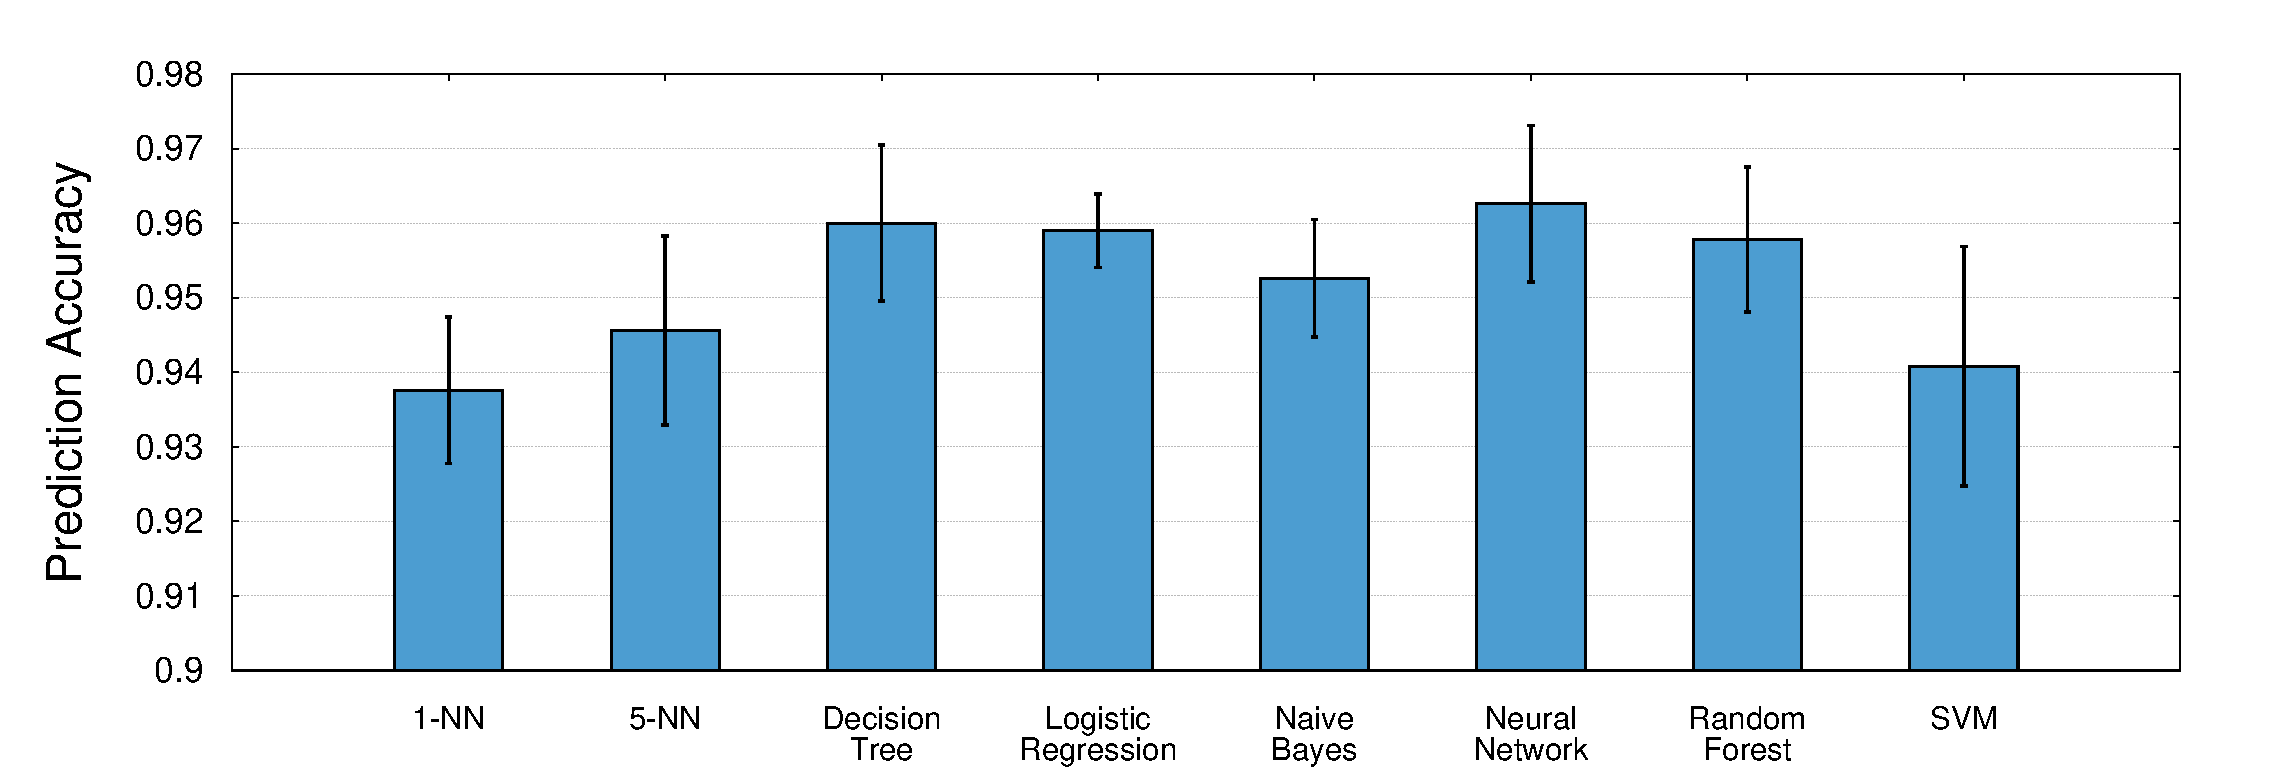
\epsfig{file=acc.eps, scale=0.45}
\caption{Average Prediction Accuracies of 8 Algorithms}
\label{fig:acc}
\end{figure*}

In Figure \ref{fig:acc}, the x-axis shows the 8 classifiers and the y-axis shows the average prediction accuracy.It is clear to see that neural network, decision tree and logistic regression have outstanding performance over the others, where neural network reaches the highest prediction accuracy and logistic regression reaches the lowest variance. Therefore, we need some other evaluation methods to select the best classifier among these three ones.

Learning curves is a good way to evaluate the performance of some certain algorithms on different sizes of training data sets. For our problem, we use $D^{(1)}$ as learning curve's data source. We still use $D_{testing}^{(1)}$ as testing data. For training, we first select $S_{hashtag} \in \{1, 2, 4, 10, 20, 50, 100, 200, 400, 800\}$ as the training data size for each of the 5 hashtags. Then when we fix $S_{hashtag}$, we randomly select $S_{hashtag}$ training tweets from $D_{training}^{(1)}$ for every hashtag and then combine them together. Thus we get a new training dataset whose size equals to $5 \times S_{hashtag}$. In similar way, we can get new training datasets with size = $\{5, 10, 20, 50, 100, 250, 500, 1000, 2000, 4000\}$. Then we can learn classifiers with these training datasets and test them with $D_{testing}^{(1)}$. Since these new training datasets are generated randomly, we repeat the process 10 times and compute the average prediction accuracy for analysis.

\begin{figure*}[!htb]
\centering
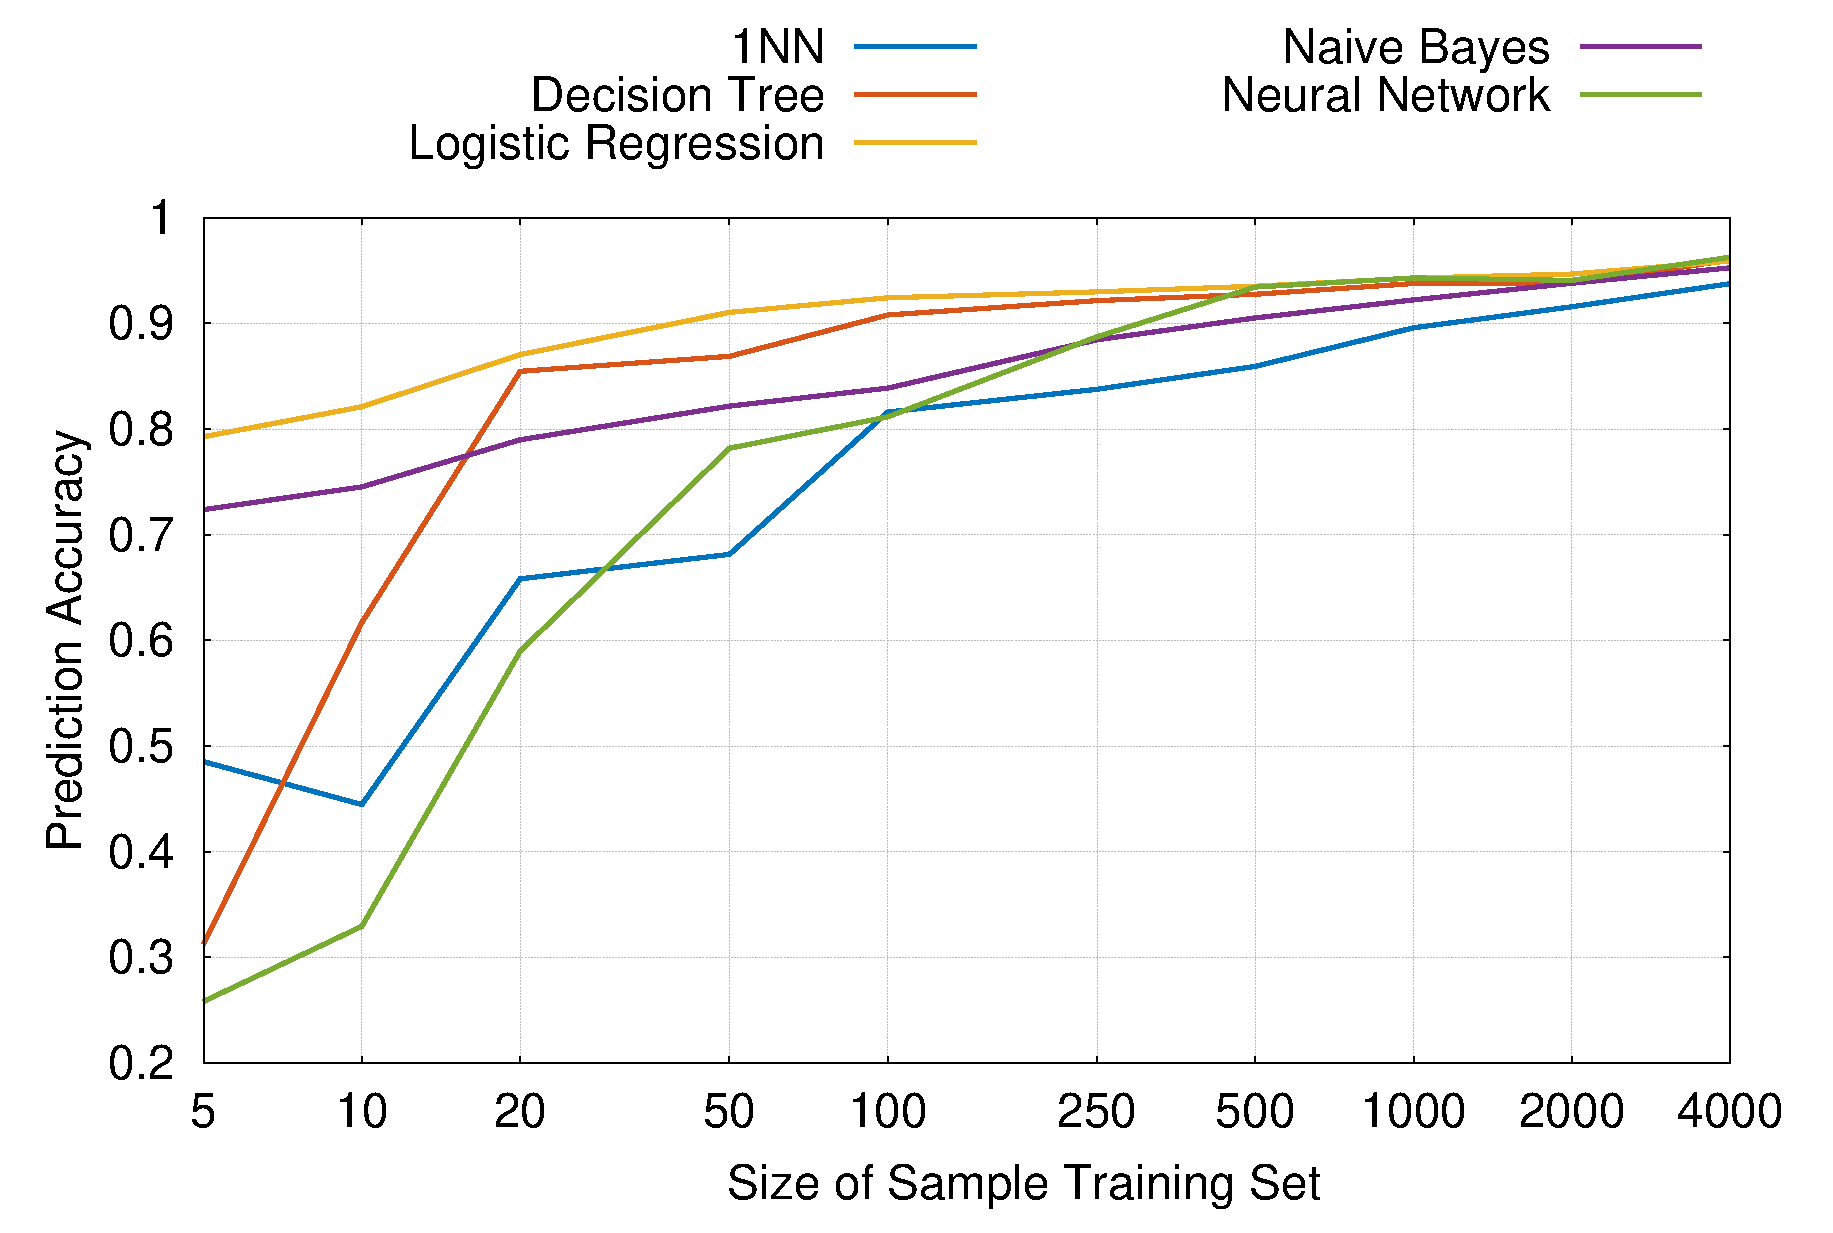
\epsfig{file=lc.eps, scale=0.50}
\caption{Learning Curve for 5 Different Algorithms}
\label{fig:lc}
\end{figure*}

Figure \ref{fig:lc} shows the prediction accuracies of 5 algorithms we have chosen in our project. Of all 5 algorithms, logistic regression and na{\"i}ve Bayes perform much better than the rest 3 ones on small training datasets. These two algorithms do rather well (roughly around 75\%) even when the training data set only contains just one training instance per topic. The rest three algorithms: decision tree, neural network and 1-NN would achieve acceptable prediction results (prediction accuracy greater than 80\%)only after the training data set has at least 20 training instances per topics. After expanding the training dataset to 200 instances per topic, all five algorithms have prediction accuracies that are greater than 90\%. 

\begin{figure*}[!htb]
\centering
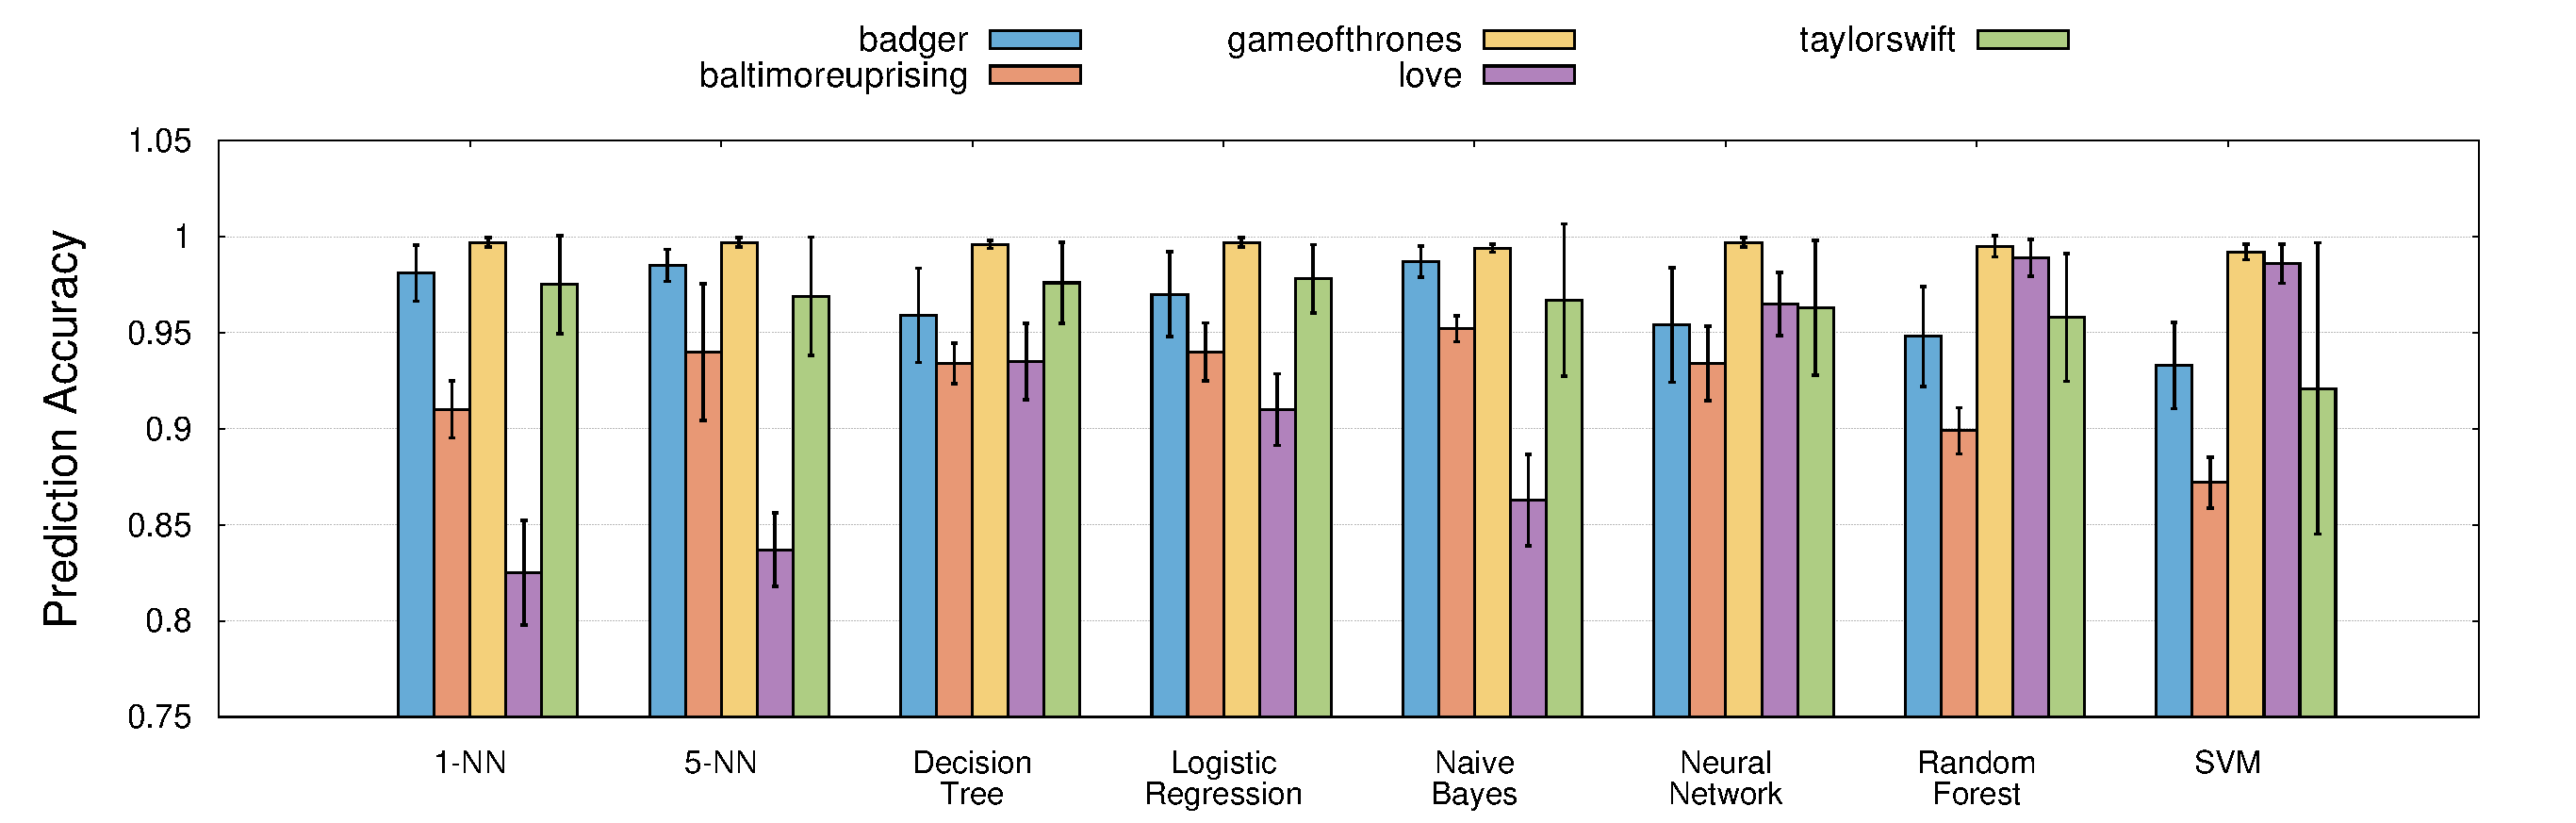
\epsfig{file=label.eps, scale=0.38}
\caption{Prediction Accuracies on 5 Different Labels}
\label{fig:lb}
\end{figure*}

From our statistic results, the hashtags chosen also have great impacts on the performances of each algorithms. Figure \ref{fig:lb} shows the average prediction accuracies of 8 different algorithms(configurations) on 5 different topics: badger, baltimoreuprising, taylorswift, gameofthrones and love. 1-NN, 5-NN, decision tree, logistic regression and na{\"i}ve Bayes have a obvious weakness in predicting love, which is to be expected, since love is a kind of common emotions that might appears in all the other topics. Surprisingly, random forest and SVM did quite well in predicting this tricky one. Topic \emph{gameofthrone} has the best prediction accuracy with almost the least stand deviation among all algorithms and configurations. The main reason why game of throne has such good result is that lots of proper noun like names of protagonists and name of places appear in almost every its related tweets, which distinguish these topic from others and therefore make predictions of this topic more accurate. Topic \emph{taylorswift} has very good average prediction accuracy but a large standard deviation as well. The major reason is that taylor-swift-related proper noun is not as many as game-of-thrones'. Some tweets might contain string implications like taylor's nick name or her songs' names so that sample datasets contains these kinds of words would have very high prediction accuracies. On the other hand, without the help of such strong implications, tweets of taylor swift are hard to distinguish with others.

Besides, we also find something interesting to address, specifically about some certain algorithm and tweets. Even if na{\"i}ve Bayes is not the implementing algorithm with best performance, it indeed draws some outstanding predictions in some cases, which shows its availability and accuracy. For example, all other implementing algorithms predicts the following tweet as \texttt{love} and only na{\"i}ve Bayes predicts it as \texttt{badgers}.
\begin{framed}
\texttt{
I may have cried when illustrating @AngelaSlatter's "Spells for Coming Forth By Daylight" http://t.co/9IMhTRLj49 \#books \#badgers \#endings
}
\end{framed}
Another thing that shall be addressed is that our dataset does have some noise. In $D^{(1)}$, we find that all implementing algorithms predict wrong for the 528th testing tweet. It shall belongs to the hashtag \texttt{gameofthrones}, but several algorithms treat it as \texttt{love}, \texttt{badgers} or \texttt{baltimoreuprising}. That's because the original content of the tweet is too simple and "common", which is
\begin{framed}
\texttt{
Yep... we've all been there. $\backslash$ud83d$\backslash$ude29 http://t.co/XTucN2D4yx  \#ILoveMondays \#Sarcasm \#GameofThrones \#GoT \#Joffrey
}
\end{framed}
It is obvious that this tweet contains no outstanding semantic terms which indicates \texttt{gameofthrones} meaning. And this case is not unique in our dataset, which affects the overall performance.

% \begin{figure*}[!htb]
% \centering
% \epsfig{file=latencies.eps, width=6.8in}
% \caption{Latencies for various IPC methods on MicroswiftOS and archlinux}
% \label{figure:latency}
% \end{figure*}

% \begin{figure*}[!htb]
% \centering
% \epsfig{file=throughput.eps, width=6.8in}
% \caption{Throughputs for various IPC methods on MicroswiftOS and archlinux}
% \label{figure:throughput}
% \end{figure*}

\section{Conclusion}
\label{sec:conc}
In this paper, we focus on testing and comparing different algorithms that can be used for tweet hashtag classification. Because our data-preparation works very well, the tweets with different hashtags have distinct feature values in our training and testing data. Therefore, all of the classifiers perform well enough. However, there are still some differences for consideration. Among these classifiers, na{\"i}ve Bayes predicts precisely in outlier cases. In general, neural network, decision trees and logistic regression perform better than the others. And logistic regression is the best one because it performs well even if the training dataset gets smaller.

% \bibliographystyle{abbrv}
\bibliographystyle{plain}
\bibliography{references}

\end{document}

% \begin{table}[!htb]
% \centering
% \begin{tabular}{|c||c|c|c|}
% \hline
% \multirow{3}{*}{\textbf{Benchmark}} & \textbf{Additional} & \textbf{Total} &\multirow{3}{*}{\textbf{Percentage}}\\ 
% &\textbf{Memory} &\textbf{Memory}&\\
% &\textbf{Accesses} &\textbf{Accesses} &\\ \hline \hline
% aster & 175481 & 2404970 & 0.0730\\ \hline 
% bzip2 & 1067380 & 9188892 & 0.1162\\ \hline 
% lbm   & 130990 & 5003775 & 0.0262\\ \hline 
% libquantum   & 54796 & 3092800 & 0.0177\\ \hline 
% milc  & 136746 & 5575859 & 0.0245\\ \hline 
% omnetpp  & 107165 & 287076 & 0.3733\\ \hline 
% \textbf{Average} & \textbf{-} &\textbf{- } &\textbf{0.1051}\\ \hline
% \end{tabular}
% \caption{Additional memory accesses for storing reuse data in a 1MB L2 reuse cache during a simulation period of 300M instructions}
% \label{table:additionalaccess}
% \end{table}

% \begin{figure}[!htb]
% \centering
% \epsfig{file=ReuseStruct.eps, height =2in, width =2in}
% \caption{Structure of our implementation for the reuse cache}
% \label{reuse:struct}
% \end{figure}

% \begin{table}[!htb]
% \centering
% \begin{tabular}{|c||c|c|c|}
% \hline
% \multirow{3}{*}{\textbf{benchmark}} & \textbf{memory} & \textbf{total} & \multirow{3}{*}{\textbf{percentage}}\\
% &\textbf{write} &\textbf{memory} &\\
% & \textbf{miss times} & \textbf{access times} & \\ \hline\hline
% bzip2 & 778893 & 16791412 & 0.0464\\ \hline 
% aster & 83555 & 4487131 & 0.0186\\ \hline 
% libquantum & 35243 & 6091860 & 0.0058\\ \hline 
% lbm & 72942 & 9862259 & 0.0074\\ \hline 
% milc & 69407 & 10820712 & 0.0064\\ \hline 
% omnetpp & 83508 & 416317 & 0.2006 \\ \hline

% \textbf{Average} &\textbf{-} &\textbf{-} &\textbf{0.0475}\\

% \hline
% \end{tabular}
% \caption{Memory write miss times in a 1MB reuse cache during a simulation period of 300M instructions}
% \label{table:writemiss}
% \end{table}



% \begin{table}[!htb]
% \centering
% \begin{tabular}{|l||r|}
% \hline
% L1 data cache size & 64KB\\
% \hline
% L1 data cache associativity & 4-way\\
% \hline
% L1 instruction cache size & 32KB\\
% \hline
% L1 instruction cache associativity & 4-way\\
% \hline
% L2 cache size & 1MB\\
% \hline
% L2 cache associativity & 8-way\\
% \hline
% Cache line size & 64B\\
% \hline
% Single memory size & 512 MB\\
% \hline
% \end{tabular}
% \caption{System configurations for baseline performance}
% \label{table:baselineconfig}
% \end{table}


% \begin{figure*}[!htb]
% \centering
% \epsfig{file=rc248.eps, width=7in}
% \caption{Relative performace of reuse cache under varying data array sizes. The data array sizes for ratio 2, 4, 8 are 512KB, 256KB, 128KB, respectively.}
% \label{fig:rc248}
% \end{figure*}



% \begin{figure}[!htb]
% \centering
% \epsfig{file=bzip2live.eps, width=3.4in}
% \caption{bzip2 percentage of live lines during execution of workload. Sampling is once per 100K data accesses.}
% \label{fig:bzip2live}
% \end{figure}

% \begin{figure*}[!htb]
% \centering
% \epsfig{file=addarray.eps, width=7in}
% \caption{Relative performace of reuse cache under varying additional block array sizes. The additional block array sizes for ratio 16, 32, 64 are 64KB, 32KB, 16KB, respectively. No additional block array means a regular reuse cache design. All statistics are obtained when reuse cache tag/data ratio is 2.}
% \label{fig:addarray}
% \end{figure*}


% \begin{table*}[!htb]
% \centering
% \begin{tabular}{|c||c|c|c|c|c|c|}
% \hline
% \multirow{2}{*}{\textbf{Benchmark}} & 
% \multicolumn{2}{c|}{\textbf{Ratio 2}} & \multicolumn{2}{c}{\textbf{Ratio 4}} & \multicolumn{2}{|c|}{\textbf{Ratio 8}}\\
% \cline{2-7}
% & \textbf{Speedup} & \textbf{Miss Rate} & \textbf{Speedup} & \textbf{Miss Rate} & \textbf{Speedup} & \textbf{Miss Rate} \\ \hline
% astar & 0.983 & 1.046 & 0.984 & 1.042 & 0.972 & 1.069\\ \hline 
% bwaves & 0.923 & 1.064 & 0.935 & 1.079 & 0.945 & 1.067\\ \hline 
% bzip2 & 0.858 & 1.114 & 0.833 & 1.112 & 0.820 & 1.154\\ \hline 
% lbm & 0.966 & 1.010 & 0.974 & 0.981 & 0.973 & 0.982\\ \hline 
% libquantum & 0.957 & 1.015 & 0.964 & 1.020 & 0.979 & 1.045\\ \hline 
% mcf & 0.876 & 1.700 & 0.833 & 2.030 & 0.796 & 2.383\\ \hline 
% milc & 0.988 & 1.016 & 0.989 & 1.021 & 0.992 & 1.014\\ \hline 
% omnetpp & 0.973 & 1.689 & 0.940 & 3.202 & 0.848 & 8.054\\ \hline 
% \textbf{Average} & \textbf{0.939} &\textbf{1.070} &\textbf{0.930} & \textbf{1.091} &\textbf{0.913} &\textbf{1.148}\\ \hline
% \end{tabular}
% \caption{Speedup and miss rate of workloads relative to baseline. Ths miss rate is a relative ratio compared with baseline miss rate.}
% \label{table:missrate}
% \end{table*}

